\documentclass[landscape,a0,final]{a0poster}

\usepackage{psfrag,graphicx,pst-grad,amsmath,amssymb,multicol,pstricks}
\usepackage{epstopdf}
\usepackage{epsfig}
\usepackage{amsmath}
\usepackage{color,graphics}
\usepackage{cite,epsfig,color,subfigure, amsthm, amssymb, mathrsfs}
\usepackage{graphicx}
\usepackage{multicol, multirow}
\usepackage{url}

% Define colour palette
\definecolor{col1}{HTML}{5A1F00}
\definecolor{col2}{HTML}{FDE792}
\definecolor{col3}{HTML}{A9CC66}
\definecolor{col4}{HTML}{D1570D}

% Do not reduce math font size in fractions etc.
\everymath{\displaystyle}

% ----------- Highlight box -------------
\newcommand{\pfbox}[4]{
\psframebox[#3]{
\begin{minipage}[t][#2][t]{#1}
#4
\end{minipage}
}}

% ---------- Figure and Table -------------
\makeatletter
\newenvironment{tablehere}
  {\def\@captype{table}}
  {}

\newenvironment{figurehere}
  {\def\@captype{figure}}
  {}
\makeatother

% ----------- Some variables --------------
\setlength{\columnsep}{3cm}
\setlength{\columnseprule}{0.5mm}
\setlength{\parindent}{0.0cm}
\topmargin -3cm
%\renewcommand{\footskip}{-2cm}
%\renewcommand{\textwidth}{81cm}
\textheight 116cm

\begin{document}
\renewcommand{\oddsidemargin}{-0.3cm}

% ---------------- Poster --------------------------------------
\begin{center}
\begin{minipage}[c]{0.99\textwidth}


% ----------------- Header -------------------------------------
\begin{center}
%% -------------------- Left logo ------------------------------
\begin{minipage}[c][6cm][c]{0.10\textwidth}
  \begin{center}
\hspace*{-5cm}
   % include logo
  \end{center}
\end{minipage}
%% -------------------- Title ------------------------------
\hspace*{-8cm}
\begin{minipage}[c][10cm][c]{0.77\textwidth}
\begin{center}
\vspace{1cm}
{\Huge {Who is P.G. Wodehouse?}}\\[0.5cm]
\hspace{0.8cm} {\Large{\textit{Wikipedia}}} \\[.5cm]
\hspace{0.5cm} {The Internet}
\end{center}
\end{minipage}
%% -------------------- Right logo ------------------------------
 \begin{minipage}[c][6cm][c]{0.13\textwidth}
   \begin{center}
     % include logo
   \end{center}
 \end{minipage}
\end{center}

\vspace*{-1cm}
\noindent\makebox[\linewidth]{\rule{\paperwidth}{0.4pt}}
% ----------------- End of Header -------------------------------

% Modify line space
\renewcommand{\baselinestretch}{1.3}

% Section title format
\newcommand{\sectitle}[1]{
\pfbox{0.98\columnwidth}{}{linecolor=col1,linewidth=0mm,fillstyle=solid,fillcolor=col1,framesep=0.8em}
{\color{white} \Large \bf #1}
}

% ------------------- Body --------------------------------------
\begin{multicols}{3}

% ------------------- Section 1 --------------------------------
\sectitle{1 \ \ Introduction}\\ \vspace*{0.5cm}

{\Large
Sir Pelham Grenville Wodehouse, KBE, (/ˈwʊdhaʊs/; 15 October 1881 – 14
February 1975) was an English humorist whose body of work includes
novels, short stories, plays, poems, song lyrics and numerous pieces
of journalism. He enjoyed enormous popular success during a career
that lasted more than seventy years, and his many writings continue to
be widely read. Despite the political and social upheavals that
occurred during his life, much of which was spent in France and the
United States, Wodehouse's main canvas remained that of a pre- and
post-World War I English upper class society, reflecting his birth,
education and youthful writing career.

An acknowledged master of English prose, Wodehouse has been admired
both by contemporaries such as Hilaire Belloc, Evelyn Waugh and
Rudyard Kipling and by recent writers such as Christopher Hitchens,
Stephen Fry,[1] Douglas Adams,[2] J. K. Rowling,[3] and John Le
Carré.[4]

Best known today for the Jeeves and Blandings Castle novels and short
stories, Wodehouse was also a playwright and lyricist who was part
author and writer of 15 plays and of 250 lyrics for some 30 musical
comedies, many of them produced in collaboration with Jerome Kern and
Guy Bolton. He worked with Cole Porter on the musical Anything Goes
(1934), wrote the lyrics for the hit song "Bill" in Kern's Show Boat
(1927), wrote lyrics to Sigmund Romberg's music for the Gershwin –
Romberg musical Rosalie (1928) and collaborated with Rudolf Friml on a
musical version of The Three Musketeers (1928). He is in the
Songwriters Hall of Fame.[5]

Wodehouse spent the last decades of his life in the United States,
becoming an American citizen in 1955, because of controversy that
arose after he made five radio broadcasts from Germany during World
War II, where he had been interned by the Germans for a
year. Speculation after the broadcasts led to allegations of
collaboration and treason. Some libraries banned his books. Although
an MI5 investigation later cleared him of any such crimes, he never
returned to England.



}
\ \\ \vspace*{0.5cm}

\begin{figurehere}
  \begin{center}
  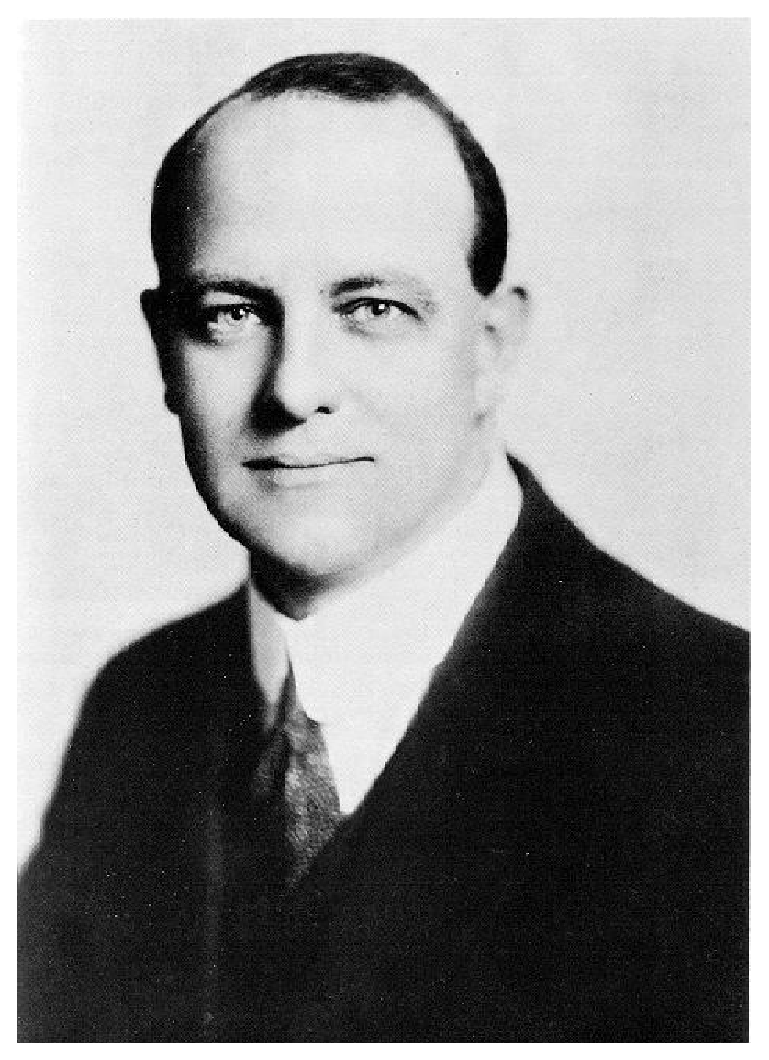
\includegraphics[scale=0.5]{PGWodehouse}
  \caption{PGW}
  \end{center}
\end{figurehere}

% ------------------- Section 2 --------------------------------
\sectitle{2 \ \ Writing Style}\\ \vspace*{0.5cm}

{\Large
Wodehouse took a modest attitude to his own works. In Over Seventy
(1957) he wrote: "I go in for what is known in the trade as 'light
writing' and those who do that – humorists they are sometimes called –
are looked down upon by the intelligentsia and sneered at."

However, he also lightly taunted his critics, as in the introduction
to Summer Lightning.[32]

A certain critic—for such men, I regret to say, do exist—made the
nasty remark about my last novel that it contained 'all the old
Wodehouse characters under different names'. He has probably by now
been eaten by bears, like the children who made mock of the prophet
Elijah; but if he still survives he will not be able to make a similar
charge against Summer Lightning. With my superior intelligence, I have
outgeneralled the man this time by putting in all the old Wodehouse
characters under the same names. Pretty silly it will make him feel, I
rather fancy.

His writing style is notable for its unique blend of contemporary
London clubroom slang with elegant, classically-informed drawing-room
English; for example:[33]

I once got engaged to his daughter Honoria, a ghastly dynamic exhibit
who read Nietzsche and had a laugh like waves breaking on a stern and
rockbound coast.[34]

Much of the charm of characters like Bertie Wooster in the
Jeeves-Wooster novels derives from the light-hearted cheeriness and
bonhomie that Wodehouse conveys through a particularly effective
choice of language. While Wooster is often described by acquaintances
as mentally negligible, the reader more often sees him as the hapless
victim of circumstances, very often circumstances which his "code",
his aspiration to be a preux chevalier (valiant knight), prevents his
avoiding. For example, Wooster is frequently made the unwilling fiancé
of girls who announce their engagement to him after discarding another
suitor. Wooster would never get out of such a fix simply by saying no,
or as he would put it, issuing a nolle prosequi, because his code does
not allow him to be so ungallant.

This is Wooster's appeal. He hasn't an ill-tempered, mean-spirited
bone in his body, and apart from some mischievous penchant for
purloining policemen's helmets, is always a gentleman. Wodehouse's
language, and Wooster's peculiar slang, neatly reinforces all of our
hero's charm. Wooster always has a nice detachment from his problems,
an ability to see them from the outside, to put himself in the third
person. Thus, he will find himself "deep in the mulligatawny with no
hope of striking for shore," "knee deep in the bisque." He will refer
to himself as B. Wooster, or Bertram, or Wooster, Bertram, and
announce that "It is pretty generally recognised by those who know him
best", and "the Woosters are always magnanimous." However others may
slight his mental acuity, or however much he may admire Jeeves for his
ability to come up with schemes to extract Wooster from the tureen, he
never loses his self-confidence, and remains convinced that he is a
man of iron will, a man who can, with the arch of an eyebrow, or
relying on just a touch of steel in his voice make others see that he
is unmoved on a given point, showing the velvet fist in the iron
glove, "if that is the phrase I want", and confident, in matters
sartorial, of his own diablerie (devilry). (Stiff Upper Lip, Jeeves,
1963)

% Wodehouse gives Wooster a rich vocabulary of slang, from abbreviated
% words, like enjoying the "b \& e" at breakfast, or "seeing at a g", to
% enjoying a drink, or lubricating the tonsils. He will describe another
% character as looking "like a seal waiting for a slice of fish," or "a
% tiger after his morning ration of coolie." He clearly enjoyed the
% benefits of a fine education at Eton and Oxford, particularly in the
% early novels, when he can spout a Shakespearean line to suit the
% occasion, or revert to the Latin citation, rem acu tetigisti, when
% putting his finger on the problem. If memory fails to bring back the
% literary reference, he can at least point Jeeves in the right
% direction: "what is that poem about someone looking at someone looking
% at something?" (Keats, "On First Looking into Chapman's Homer".) It is
% only in the later stories that he loses his smattering of learning,
% and attributes the most familiar Shakespearian quotations to
% Jeeves. Wodehouse's use of language was outstanding, including coining
% new words. "[W]hile not actually disgruntled, he was far from being
% gruntled".

}

\end{multicols}
% ------------------- End of Body ----------------------------
\end{minipage} 
\end{center}
% ------------------- End of Poster ---------------------------
\end{document}
